%% A/C differences

In the first iteration of the analysis, a large discrepancy between the two endcaps (A-side and C-side) was observed in several forward $\eta$ bins in the events satisfying W selection (Fig.~\ref{fig:Wmunu:AC_old_W}). This discrepancy was not seen in Z events (Fig.~\ref{fig:Wmunu:AC_old_Z}).

\begin{figure}[phtb]
  \begin{center}
        \subfigure[\Wminus]{%
	  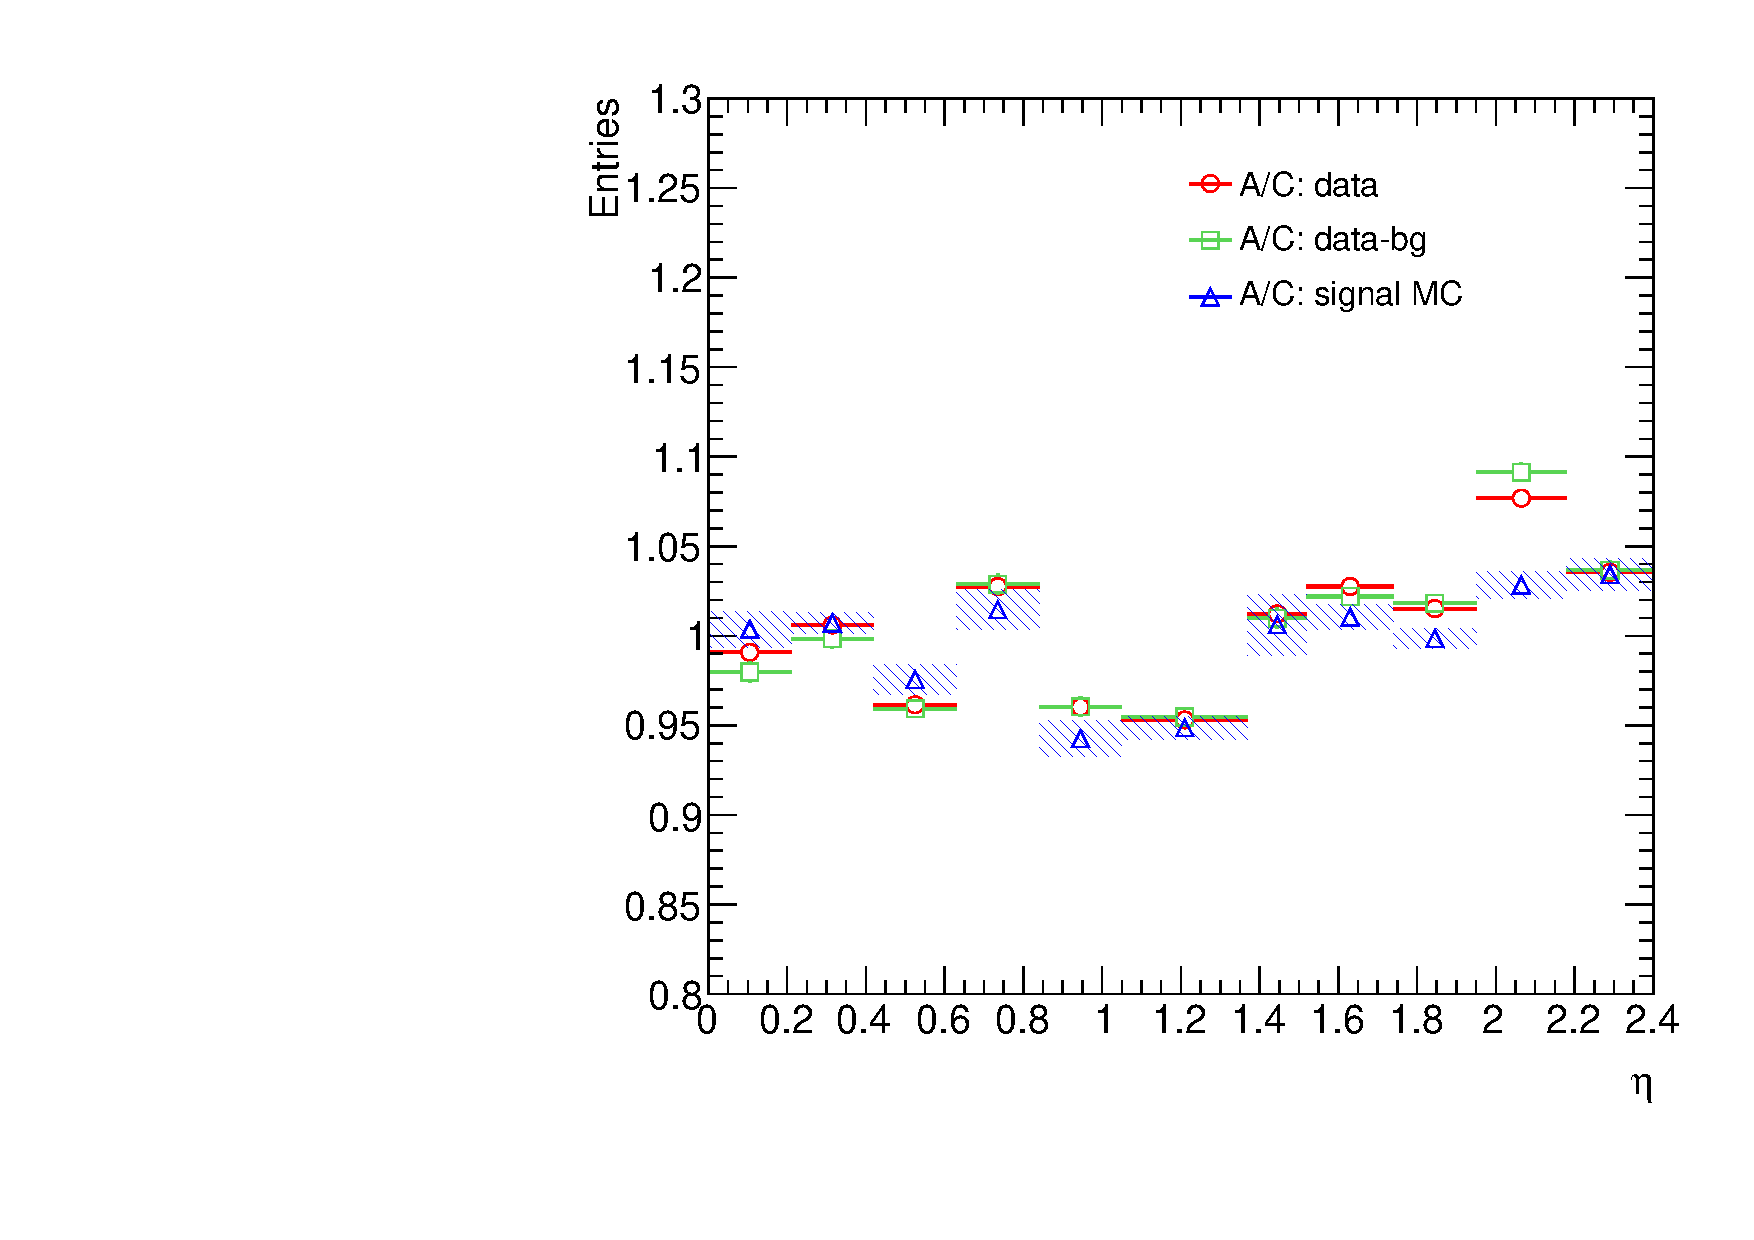
\includegraphics[width=0.45\textwidth]{event/AC/old/W_NOM_Q0_stack_d3_eta_lpt_met_y_2__1_z_0__1_NEG}
        }
        \subfigure[\Wplus]{%
	  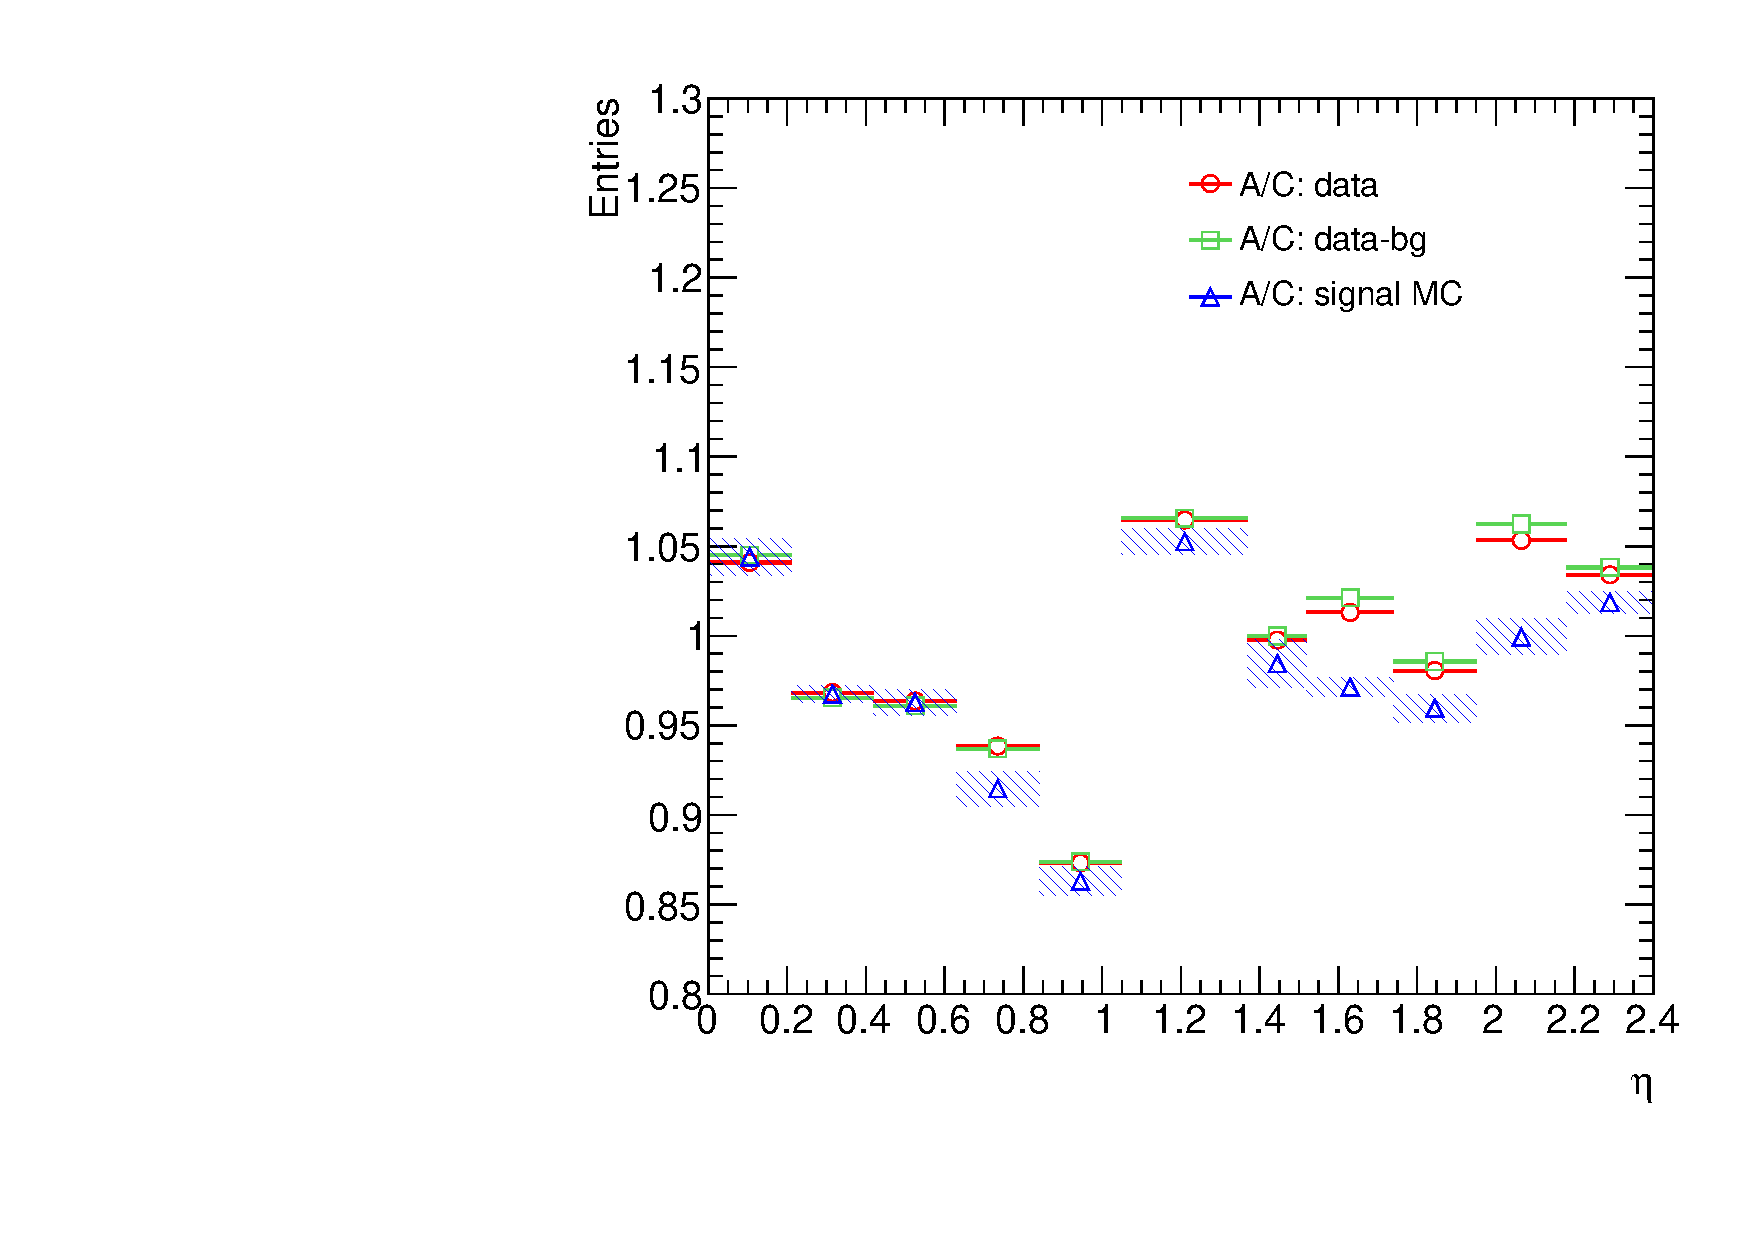
\includegraphics[width=0.45\textwidth]{event/AC/old/W_NOM_Q0_stack_d3_eta_lpt_met_y_2__1_z_0__1_POS}
        }
 \caption{ Forward-$\eta$ discrepancy in the A/C ratio at the detector level for events satisfying W selection (muGirl trigger). Shaded error bands include all systematics, which are propagated coherently to form the A-to-C ratio. In these plots, signal is Powheg+Pythia and QCD is estimated from heavy-flavor Monte-Carlo. }
 \label{fig:Wmunu:AC_old_W}
 \end{center}
\end{figure}

\begin{figure}[phtb]
  \begin{center}
        \subfigure[Z, $\mu^-$ only]{%
	  \includegraphics[width=0.45\textwidth]{Wmunu/figures/AC/old/ZNT_TMATCHBOTH_stack_leptonN_etav_ALL}
        }
        \subfigure[Z, $\mu^+$ only]{%
	  \includegraphics[width=0.45\textwidth]{Wmunu/figures/AC/old/ZNT_TMATCHBOTH_stack_leptonP_etav_ALL}
        }
 \caption{ A/C ratio at the detector level for muons in di-muon events satisfying Z selection (mu18\_MG). Note nearly perfect agreement in forward $\eta$ bins. In these plots, signal is Powheg+Pythia. Both reconstructed muons are required to match to an event-filter trigger object. Only one muon per event (depending on the charge) enters each plot. Due to small backgrounds in the Z boson selection, the greed points (data-bg) appear superimposed on the red points (data only). }
 \label{fig:Wmunu:AC_old_Z}
 \end{center}
\end{figure}

The following potential sources of this discrepancy were examined and excluded:
\begin{itemize}
\item Muon-specific terms in missing energy calculation
\item Calorimeter terms in missing energy calculation
\item Overall definition of missing energy (RefFinal vs LocHadTopo)
\item Muon momentum and resolution corrections
\item Muon quality cuts (such as the difference between ID and MS $p_T$ measurements)
\item Impact parameter cut
\item Trigger matching cone size
\item Kinematic cuts, such as transverse mass or muon momentum
\item Binning of scale factors
\item Relaxing or dropping the di-muon mass constraint in Z selection
\item Trying to narrow the problem to a particular $\phi$ quadrant
\end{itemize}

Several observations suggested that the problem is related to the muon trigger.

Figures~\ref{fig:Wmunu:AC_eta_POS_8}~-~\ref{fig:Wmunu:AC_eta_POS_10} zoom inside inside the three measurement bins with a large A/C discrepancy. For comparison, Fig.~\ref{fig:Wmunu:AC_eta_POS_7} repeats the same plots inside one of the ``good'' bins. A large A/C discrepancy is always associated with a narrow $\eta$ dip in efficiency in data for events satisfying W selection. These dips are not modeled by Monte-Carlo and, surprisingly, are not seen in events satisfying Z selection. In contrast, the ``good'' bins (as far as the A/C discrepancy goes) sometimes also have efficiency dips, but those dips are always reproduced in Z selection (Fig.~\ref{fig:Wmunu:AC_eta_POS_7}).

\begin{figure}[phtb]
  \begin{center}
        \subfigure[W, $\mu^+$, $1.52<|\eta|<1.74$, C-side]{%
	  \includegraphics[width=0.45\textwidth]{Wmunu/figures/AC/eta/W_8_C_stack_l_eta_POS}
        }
        \subfigure[W, $\mu^+$, $1.52<|\eta|<1.74$, A-side]{%
	  \includegraphics[width=0.45\textwidth]{Wmunu/figures/AC/eta/W_8_A_stack_l_eta_POS}
        } \\
        \subfigure[Z, $\mu^+$, $1.52<|\eta|<1.74$, C-side]{%
	  \includegraphics[width=0.45\textwidth]{Wmunu/figures/AC/eta/Z_8_C_stack_lP_eta_ALL}
        }
        \subfigure[Z, $\mu^+$, $1.52<|\eta|<1.74$, A-side]{%
	  \includegraphics[width=0.45\textwidth]{Wmunu/figures/AC/eta/Z_8_A_stack_lP_eta_ALL}
        }
 \caption{ $\mu^+$ $\eta$ distributions for W and Z candidates inside the 8th $|\eta|$ bin ($1.52<|\eta|<1.74$). A dip is seen on the C-side, but only in W events.}
 \label{fig:Wmunu:AC_eta_POS_8}
 \end{center}
\end{figure}


\begin{figure}[phtb]
  \begin{center}
        \subfigure[W, $\mu^-$, $1.95<|\eta|<2.18$, C-side]{%
	  \includegraphics[width=0.45\textwidth]{Wmunu/figures/AC/eta/W_10_C_stack_l_eta_NEG}
        }
        \subfigure[W, $\mu^-$, $1.95<|\eta|<2.18$, A-side]{%
	  \includegraphics[width=0.45\textwidth]{Wmunu/figures/AC/eta/W_10_A_stack_l_eta_NEG}
        } \\
        \subfigure[Z, $\mu^-$, $1.95<|\eta|<2.18$, C-side]{%
	  \includegraphics[width=0.45\textwidth]{Wmunu/figures/AC/eta/Z_10_C_stack_lN_eta_ALL}
        }
        \subfigure[Z, $\mu^-$, $1.95<|\eta|<2.18$, A-side]{%
	  \includegraphics[width=0.45\textwidth]{Wmunu/figures/AC/eta/Z_10_A_stack_lN_eta_ALL}
        }
 \caption{ $\mu^-$ $\eta$ distributions for W and Z candidates inside the 10th $|\eta|$ bin ($1.95<|\eta|<2.18$). A dip is seen on the C-side, but only in W events.}
 \label{fig:Wmunu:AC_eta_NEG_10}
 \end{center}
\end{figure}

\begin{figure}[phtb]
  \begin{center}
        \subfigure[W, $\mu^+$, $1.95<|\eta|<2.18$, C-side]{%
	  \includegraphics[width=0.45\textwidth]{Wmunu/figures/AC/eta/W_10_C_stack_l_eta_POS}
        }
        \subfigure[W, $\mu^+$, $1.95<|\eta|<2.18$, A-side]{%
	  \includegraphics[width=0.45\textwidth]{Wmunu/figures/AC/eta/W_10_A_stack_l_eta_POS}
        } \\
        \subfigure[Z, $\mu^+$, $1.95<|\eta|<2.18$, C-side]{%
	  \includegraphics[width=0.45\textwidth]{Wmunu/figures/AC/eta/Z_10_C_stack_lP_eta_ALL}
        }
        \subfigure[Z, $\mu^+$, $1.95<|\eta|<2.18$, A-side]{%
	  \includegraphics[width=0.45\textwidth]{Wmunu/figures/AC/eta/Z_10_A_stack_lP_eta_ALL}
        }
 \caption{ $\mu^+$ $\eta$ distributions for W and Z candidates inside the 10th $|\eta|$ bin ($1.95<|\eta|<2.18$). A dip is seen on the C-side, but only in W events. Also note that the location of the dip is slightly offset (in $\eta$) with respect to the negative muons. }
 \label{fig:Wmunu:AC_eta_POS_10}
 \end{center}
\end{figure}

\begin{figure}[phtb]
  \begin{center}
        \subfigure[W, $\mu^+$, $1.37<|\eta|<1.52$, C-side]{%
	  \includegraphics[width=0.45\textwidth]{Wmunu/figures/AC/eta/W_7_C_stack_l_eta_POS}
        }
        \subfigure[W, $\mu^+$, $1.37<|\eta|<1.52$, A-side]{%
	  \includegraphics[width=0.45\textwidth]{Wmunu/figures/AC/eta/W_7_A_stack_l_eta_POS}
        } \\
        \subfigure[Z, $\mu^+$, $1.37<|\eta|<1.52$, C-side]{%
	  \includegraphics[width=0.45\textwidth]{Wmunu/figures/AC/eta/Z_7_C_stack_lP_eta_ALL}
        }
        \subfigure[Z, $\mu^+$, $1.37<|\eta|<1.52$, A-side]{%
	  \includegraphics[width=0.45\textwidth]{Wmunu/figures/AC/eta/Z_7_A_stack_lP_eta_ALL}
        }
 \caption{ $\mu^+$ $\eta$ distributions for W and Z candidates inside the 7th $|\eta|$ bin ($1.37<|\eta|<1.52$). This bin does not exhibit a large A/C discrepancy, but still has a dip. However, unlike the 8th and 10th bins, the dip in this case is reproduced in Z selection. }
 \label{fig:Wmunu:AC_eta_POS_7}
 \end{center}
\end{figure}

These efficiency dips are not present in early data taking and only appear after the technical stop between periods H and I. For example, Fig.~\ref{fig:Wmunu:AC_period} zooms on the $1.95<|\eta|<2.18$ bin for periods D-H only, and for period I only. Note that the appearance of the dips doesn't quite coincide with the switch from mu18\_MG to mu18\_MG\_medium trigger, which occurred starting with period J.

\begin{figure}[phtb]
  \begin{center}
        \subfigure[Periods D-H only: \Wminus, $1.95<|\eta|<2.18$, C-side]{%
	  \includegraphics[width=0.45\textwidth]{Wmunu/figures/AC/old/WpDtoH_10_C_stack_l_eta_NEG}
        }
        \subfigure[Period I only: \Wminus, $1.95<|\eta|<2.18$, C-side]{%
	  \includegraphics[width=0.45\textwidth]{Wmunu/figures/AC/old/WpItoI_10_C_stack_l_eta_NEG}
        }
 \caption{ Efficiency dips seen in W but not Z events are only present in later data periods. Here, this is shown explicitly for \Wminus\ events in the $1.95<|\eta|<2.18$ bin.}
 \label{fig:Wmunu:AC_period}
 \end{center}
\end{figure}

Figures~\ref{fig:Wmunu:AC_mu18_POS_8}-~\ref{fig:Wmunu:AC_mu18_POS_10} show that the efficiency dips seen in W but not Z events disappear entirely if the muid family of triggers (mu18 and mu18\_medium) is used instead of the muGirl family (mu18\_MG and mu18\_MG\_medium). A more comprehensive study of inefficiencies associated with the muGirl triggers is shown in Fig.~\ref{fig:Wmunu:AC_MGvsMU}, which plots 2D histograms ($\eta-\phi$) of events for which the muid trigger succeeds but muGirl fails, for two different data periods. The muGirl triggers clearly have a serious problem on the C-side that was introduced in later data-taking periods.

\begin{figure}[phtb]
  \begin{center}
        \subfigure[muGirl triggers: \Wplus, $1.52<|\eta|<1.74$, C-side]{%
	  \includegraphics[width=0.45\textwidth]{Wmunu/figures/AC/old/WMU18_MG_8_C_stack_l_eta_POS}
        }
        \subfigure[muid triggers: \Wplus, $1.52<|\eta|<1.74$, C-side]{%
	  \includegraphics[width=0.45\textwidth]{Wmunu/figures/AC/old/WMU18_8_C_stack_l_eta_POS}
        }
 \caption{ Efficiency dips seen in W but not Z events are only present with the muGirl triggers (mu18\_MG and mu18\_MG\_medium). They disappear when muid triggers are used (mu18 and mu18\_medium). Here, this is shown explicitly for \Wplus\ events in the $1.52<|\eta|<1.74$ bin. }
 \label{fig:Wmunu:AC_mu18_POS_8}
 \end{center}
\end{figure}

\begin{figure}[phtb]
  \begin{center}
        \subfigure[muGirl triggers: \Wminus, $1.95<|\eta|<2.18$, C-side]{%
	  \includegraphics[width=0.45\textwidth]{Wmunu/figures/AC/old/WMU18_MG_10_C_stack_l_eta_NEG}
        }
        \subfigure[muid triggers: \Wminus, $1.95<|\eta|<2.18$, C-side]{%
	  \includegraphics[width=0.45\textwidth]{Wmunu/figures/AC/old/WMU18_10_C_stack_l_eta_NEG}
        }
 \caption{ Efficiency dips seen in W but not Z events are only present with the muGirl triggers (mu18\_MG and mu18\_MG\_medium). They disappear when muid triggers are used (mu18 and mu18\_medium). Here, this is shown explicitly for \Wminus\ events in the $1.95<|\eta|<2.18$ bin. }
 \label{fig:Wmunu:AC_mu18_NEG_10}
 \end{center}
\end{figure}

\begin{figure}[phtb]
  \begin{center}
        \subfigure[muGirl triggers: \Wplus, $1.95<|\eta|<2.18$, C-side]{%
	  \includegraphics[width=0.45\textwidth]{Wmunu/figures/AC/old/WMU18_MG_10_C_stack_l_eta_POS}
        }
        \subfigure[muid triggers: \Wplus, $1.95<|\eta|<2.18$, C-side]{%
	  \includegraphics[width=0.45\textwidth]{Wmunu/figures/AC/old/WMU18_10_C_stack_l_eta_POS}
        }
 \caption{ Efficiency dips seen in W but not Z events are only present with the muGirl triggers (mu18\_MG and mu18\_MG\_medium). They disappear when muid triggers are used (mu18 and mu18\_medium). Here, this is shown explicitly for \Wplus\ events in the $1.95<|\eta|<2.18$ bin. }
 \label{fig:Wmunu:AC_mu18_POS_10}
 \end{center}
\end{figure}

\begin{figure}[phtb]
  \begin{center}
        \subfigure[period D, \Wminus]{%
	  \includegraphics[width=0.45\textwidth]{Wmunu/figures/AC/old/dump_MG_dataD_w_NEG.dat__MUID_NOT_MG}
        }
        \subfigure[period D, \Wplus]{%
	  \includegraphics[width=0.45\textwidth]{Wmunu/figures/AC/old/dump_MG_dataD_w_POS.dat__MUID_NOT_MG}
        } \\
        \subfigure[period L, \Wminus]{%
	  \includegraphics[width=0.45\textwidth]{Wmunu/figures/AC/old/dump_MG_dataL_w_NEG.dat__MUID_NOT_MG}
        }
        \subfigure[period L, \Wplus]{%
	  \includegraphics[width=0.45\textwidth]{Wmunu/figures/AC/old/dump_MG_dataL_w_POS.dat__MUID_NOT_MG}
        }
 \caption{ Events satisfying standard W selection that pass the muid triggers but fail muGirl triggers, shown separately for an early data period (period D) and a later one (period L). A large additional inefficiency is introduced by the muGirl triggers in later data periods. }
 \label{fig:Wmunu:AC_MGvsMU}
 \end{center}
\end{figure}

A localized inefficiency in muGirl triggers would normally be corrected by the tag-and-probe trigger scale factors. However, events satisfying Z selection do not exhibit these efficiency dips - even if both muons are required to match to an EF trigger object. Such localized inefficiencies evade tag-and-probe corrections. The hypothesis is that the trigger matching machinery does not work correctly for MG trigger chains. More specifically, asking for a cone match to an EF muGirl object does not necessarily imply that a muon satisfied the trigger condition in hardware. In Z events, this means that the requirement for the plotted probe muon to ``match'' the trigger may not be doing what we think (at least in specific $\eta$ regions). This can mask an actual trigger inefficiency when the probe muons falls in these $\eta$ regions because the event can still be triggered by the tag muon. On the other hand, events without a second muon (such as those that satisfy the W selection) do not have a second muon to fall back on, so any localized trigger inefficiency becomes manifest.

In an attempt to ``fix'' muGirl trigger matching and reproduce efficiency dips in Z events, the matching was repeated with two different software packages: ``TrigMuonEfficiency'', which is recommended for the end users, and ``TrigMatchTool'', which operates on more basic objects in the ntuple and is normally reserved for the experts. With either package, the efficiency dips in Z probe events failed to appear, pointing to a more fundamental problem with the trigger matching machinery when it comes to muGirl triggers.

Fig.~\ref{fig:Wmunu:AC_tfail} considers a subsample of Z events where the tag muon is explicitly forced to fail the trigger, which is not an uncommon situation as some regions of the detector are not instrumented with muon trigger chambers. This implicitly forces the probe muon to be the muon that triggered the event. In this case, events with Z selection recover the same efficiency dip seen in W selection.

\begin{figure}[phtb]
  \begin{center}
        \subfigure[Z: both legs match to trigger, $\mu^-$ ]{%
	  \includegraphics[width=0.30\textwidth]{Wmunu/figures/AC/old/Z_10_C_stack_lN_eta_ALL}
        }
        \subfigure[Z: tag fails trigger match, $\mu^-$ ]{%
	  \includegraphics[width=0.30\textwidth]{Wmunu/figures/AC/old/Ztinv_10_C_stack_lN_eta_ALL}
        }
        \subfigure[W, $\mu^-$ ]{%
	  \includegraphics[width=0.30\textwidth]{Wmunu/figures/AC/old/W_10_C_stack_l_eta_NEG}
        }
 \caption{ When the tag muon is forced to fail trigger match (center), the probe muon is implicitly forced to be the muon that triggered the event. In this case, events with Z selection recover the same efficiency dip around $\eta=-2.08$ as seen in the W selection (right). }
 \label{fig:Wmunu:AC_tfail}
 \end{center}
\end{figure}

In summary, the muGirl trigger chains suffer from a sizable inefficiency on the C-side, which cannot be corrected with Z tag-and-probe trigger scale factors because trigger matching to muGirl EF-level objects does not work correctly in some $\eta$ regions. These issues were reported to relevant experts.

Because the muid triggers are not affected by the aforementioned problems, they were chosen over the muGirl family for both the \Wmn\ and \Zmm\ channels. Fig.~\ref{fig:Wmunu:AC_new_W} shows that the large A/C discrepancies seen previously in some forward $\eta$ bins are gone when using the muid triggers.

\begin{figure}[phtb]
  \begin{center}
        \subfigure[\Wminus]{%
	  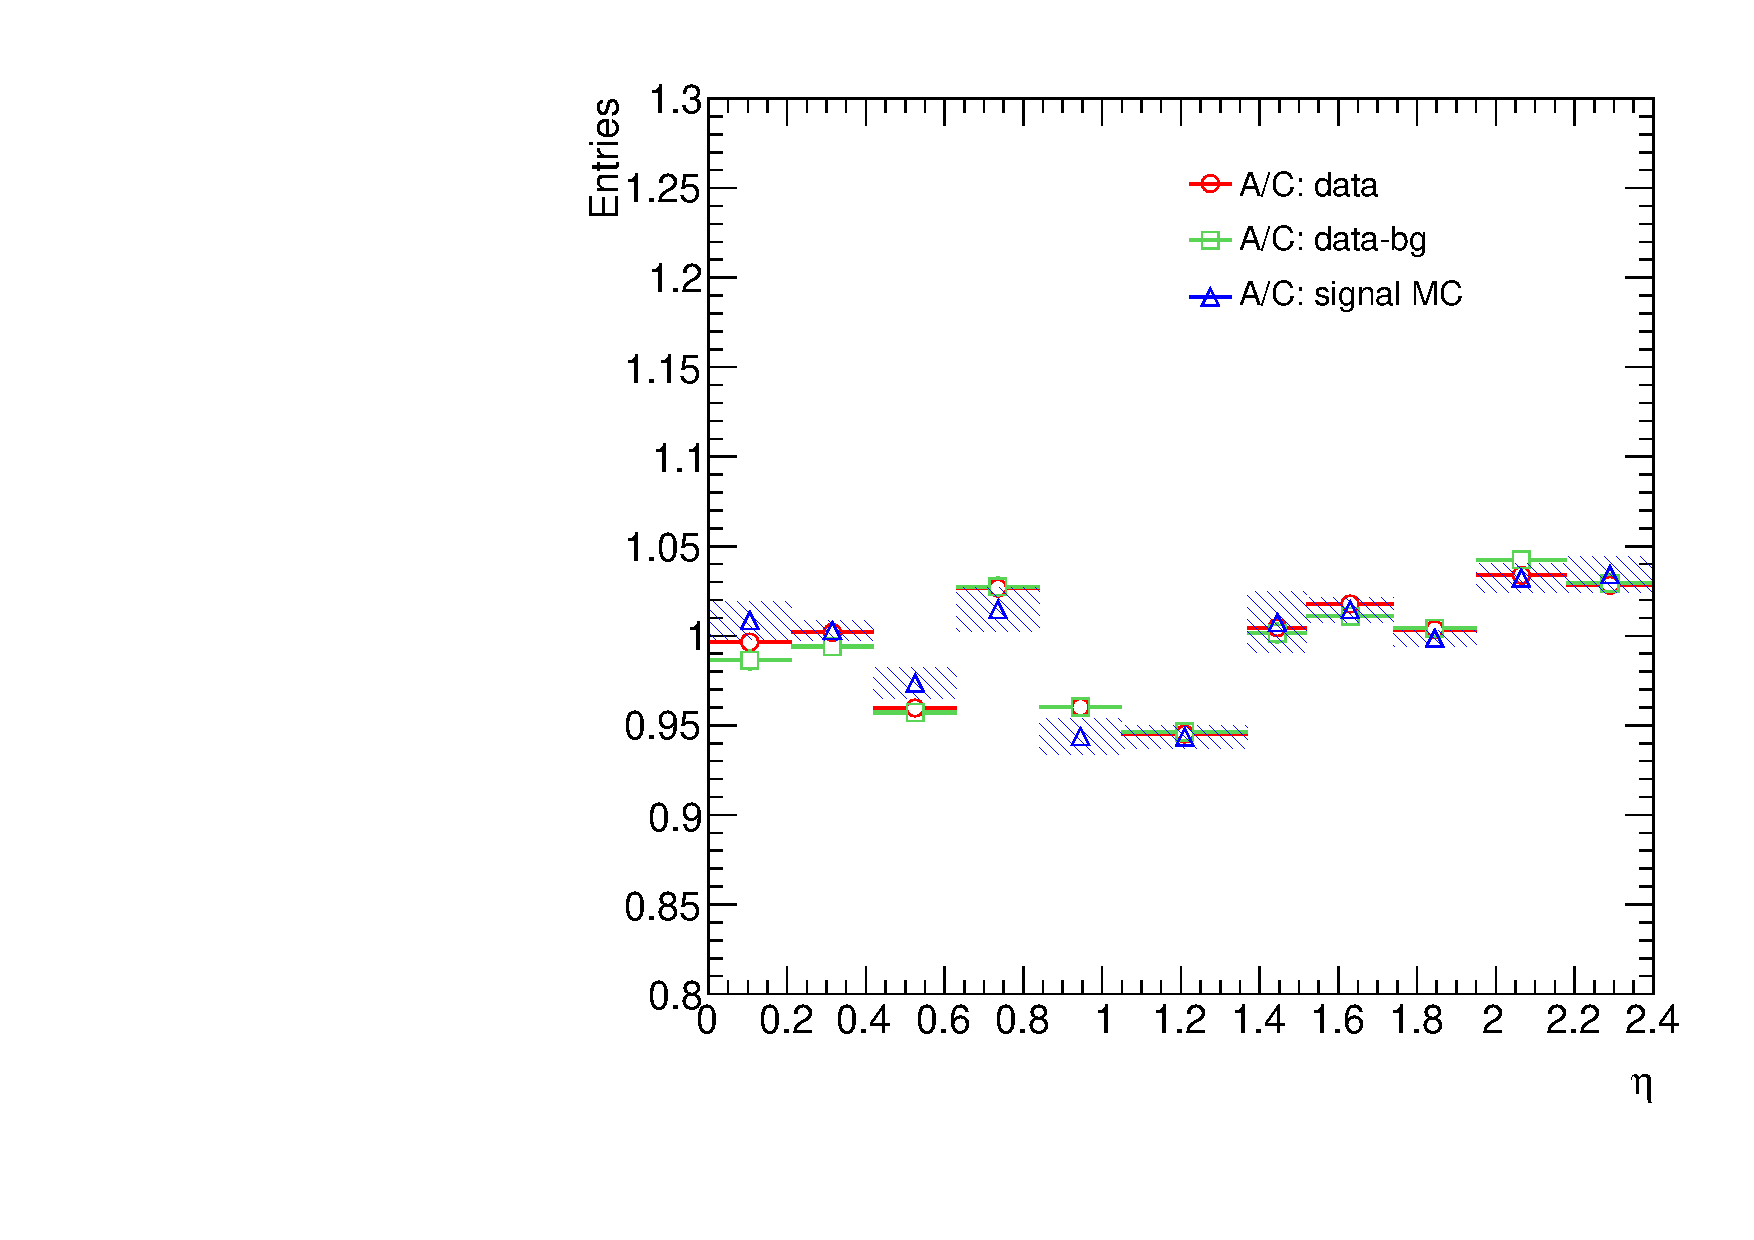
\includegraphics[width=0.45\textwidth]{event/AC/new/W_NOM_Q0_stack_d3_eta_lpt_met_y_2__1_z_0__1_NEG}
        }
        \subfigure[\Wplus]{%
	  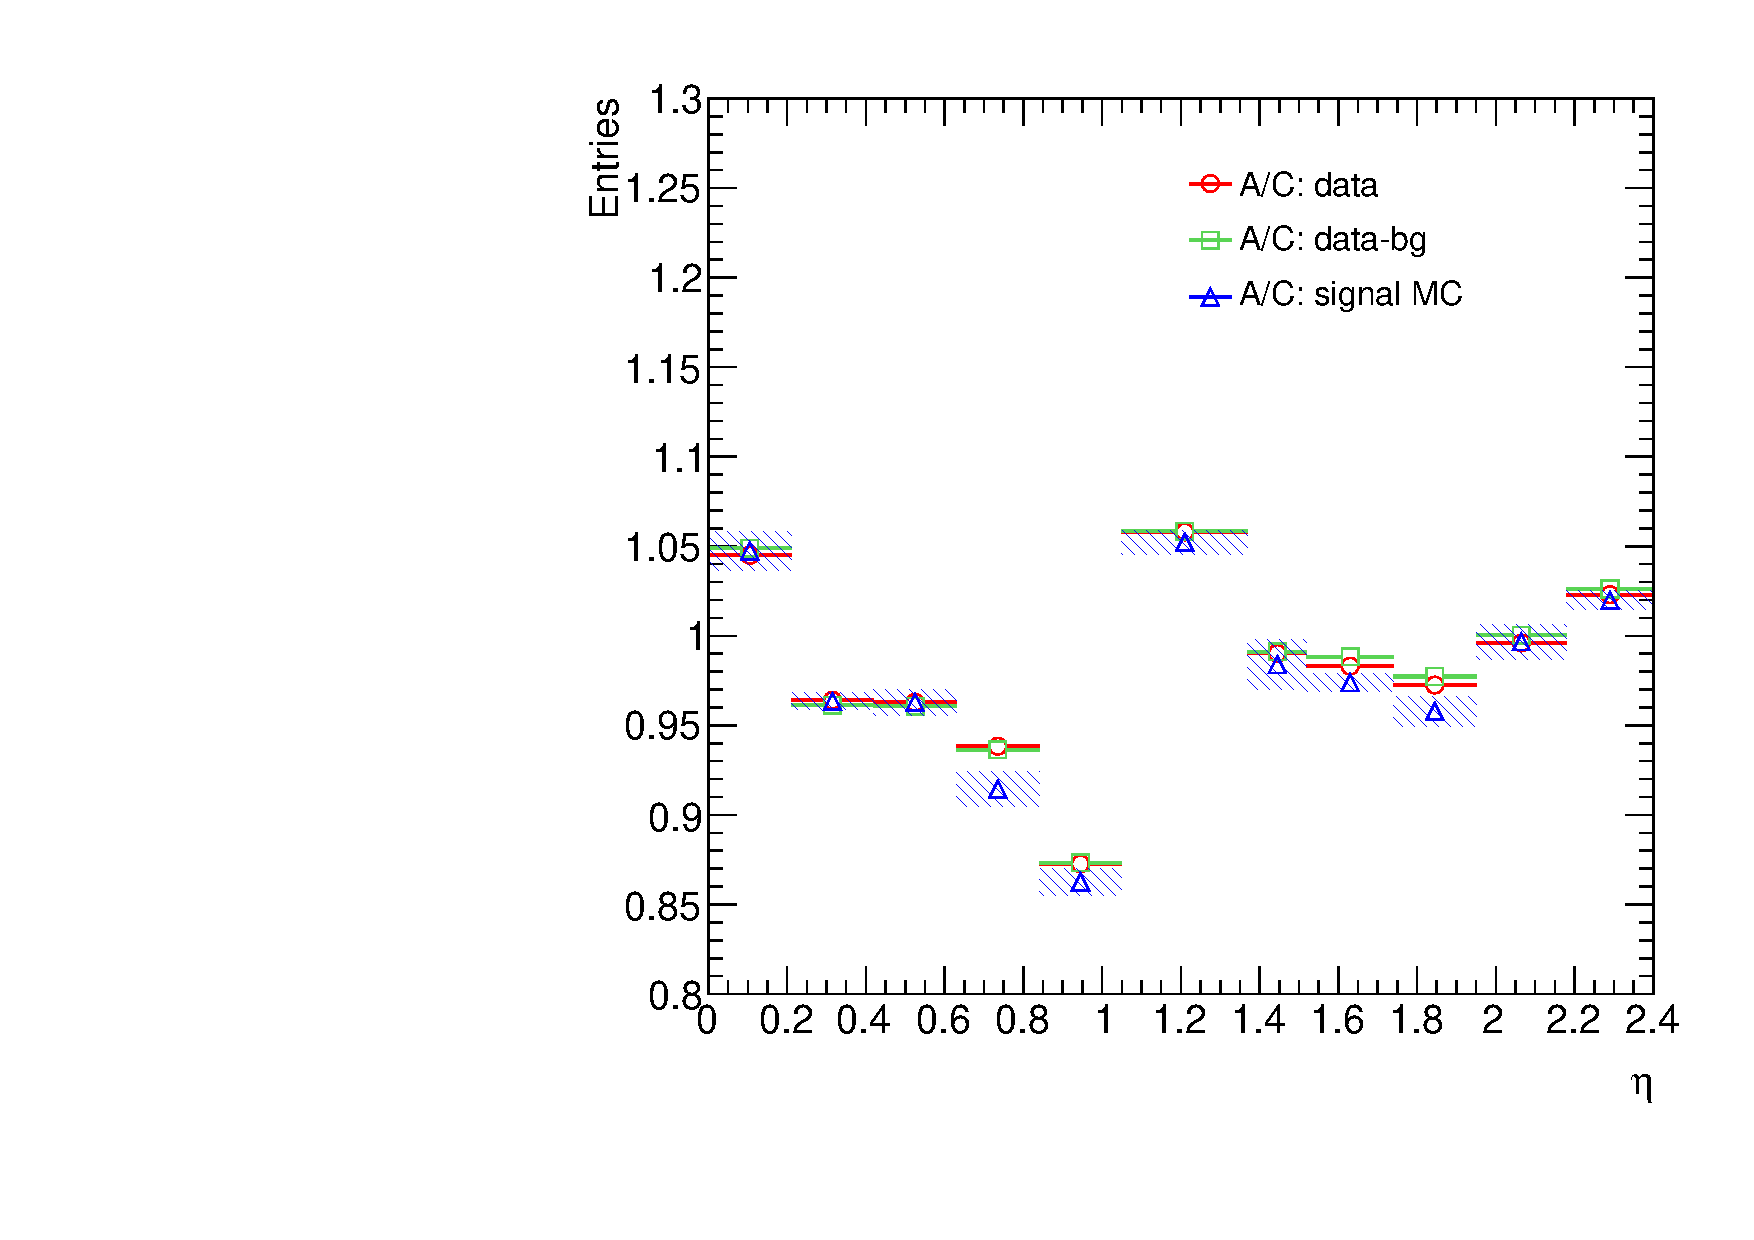
\includegraphics[width=0.45\textwidth]{event/AC/new/W_NOM_Q0_stack_d3_eta_lpt_met_y_2__1_z_0__1_POS}
        }
 \caption{ The large discrepancies in A/C ratio are not seen with the muid trigger chains. Shaded error bands include all systematics, which are propagated coherently to form the A-to-C ratio. In these plots, signal is Powheg+Pythia and QCD is estimated from heavy-flavor Monte-Carlo. }
 \label{fig:Wmunu:AC_new_W}
 \end{center}
\end{figure}

% mu-: 1866.344  ->  1874.673
% mu+: 2779.197  ->  2799.126
As a result of switching the trigger to muid chains, the measured value of the integrated cross-section increased by 0.5\% for $\mu^-$ and 0.7\% for $\mu^+$, consistent with the fact that the muGirl chains have localized inefficiencies in data that cannot be recovered with Z tag-and-probe.
